\section{Aufbau und Durchführung}
\label{sec:Aufbau und Durchführung}

\subsection{Messung der Hysteresekurve}
Für die Messung der Hysteresekurve wird Abbildung \eqref{fig:Hall-Aufbau}, ohne den Hallapparat aufgebaut.

\begin{figure}[H]
  \centering
  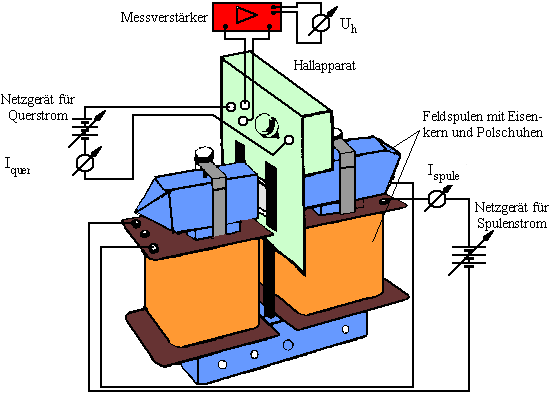
\includegraphics[height=7cm]{picture/Hall-Aufbau.png}
  \caption{Versuchsaufbau zur Messung der Hall-Spannung. \cite{LEIFI}}
  \label{fig:Hall-Aufbau}
\end{figure}

Nun wird der Spulenstrom in 10 äquidistanten Schritten von 0\,A auf 5\,A gedreht und zu jedem Wert wird das Magnetfeld, mit Hilfe einer Hall-Sonde gemessen. Danach wird der Spulenstrom in den gleichen Schritten nach unten gedreht und wieder das Magnetfeld gemessen. Die gemessenen Werte werden nun in einem Diagramm aufgetragen.

\subsection{Messung der Hall-Spannung}
Für die Messung der Hall-Spannung wird Abbildung \eqref{fig:Hall-Aufbau} aufgebaut. Der Spulenstrom wird auf 5\,A gedreht und der Querstrom in äquidistanten Schritten nach oben gedreht. Die Hall-Spannung wird für jeden Querstrom auf einem digital Voltmeter ausgegeben und notiert.

\subsection{Messung des elektrischen Widerstandes}
Zur Messung des elektrischen Widerstandes wird der in Abbildung \eqref{fig:Hall-Effekt1} gezeigte Aufbau modifiziert.

\begin{figure}[H]
	\centering
	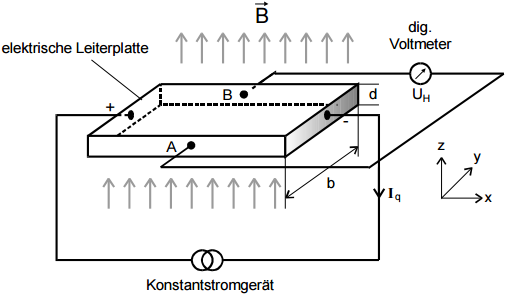
\includegraphics[height=7cm]{picture/Hall-Effekt.png}
	\caption{Schematischer Aufbau zur Beobachtung des Hall-Effektes. \cite[5]{sample}}
	\label{fig:Hall-Effekt1}
\end{figure}

Statt der Hall-Spannung wird die Spannung, welche auf der x-Achse der Leiterplatte anliegt gemessen. Dies wird für 10 unterschiedliche Querströme gemacht und die jeweilige Spannung wird notiert.  
